% CHAPTER 6: SYSTEM ARCHITECTURE
\chapter{System Architecture}

The RespiraTech system architecture will consist of four major layers working together to deliver AI-driven disease prediction from breath analysis. This chapter describes each layer, their individual responsibilities, and their interconnections.

\section{System Block Diagram}

The system architecture is organized into four distinct layers:

\begin{enumerate}[leftmargin=1.5cm]
\item \textbf{Sensing Layer:} Gas sensors (MQ-135, MQ-3) and environmental sensor (DHT11/DHT22) mounted inside the breath collection chamber.
\item \textbf{Edge Processing Layer:} ESP32 microcontroller performing ADC sampling, feature extraction, and Wi-Fi data transmission.
\item \textbf{Cloud Intelligence Layer:} Cloud platform (ThingSpeak/Firebase) hosting the data pipeline and ML inference engine.
\item \textbf{Presentation Layer:} Mobile/web application and OLED display delivering health risk predictions to the user.
\end{enumerate}

Data flows upward from the Sensing Layer through the Edge Processing and Cloud Intelligence Layers, with prediction results flowing back down to the Presentation Layer. The OLED display provides local feedback directly from the Edge Processing Layer, while the mobile/web app retrieves results from the Cloud Intelligence Layer.

\section{Power Supply Subsystem}
The power supply subsystem will provide regulated power to all system components. It consists of the following elements:

\begin{itemize}[leftmargin=1.5cm]
\item \textbf{USB 5V Input / LiPo Battery:} The primary power source will be either a USB 5V connection (for stationary use) or a 3.7V, 2000 mAh lithium polymer battery with a TP4056 USB charging module (for portable use). The TP4056 will provide safe CC/CV charging with automatic cutoff at 4.2V and undervoltage protection at 2.5V.

\item \textbf{Voltage Regulation:} The ESP32's onboard AMS1117-3.3V regulator will convert the 5V USB or battery input to 3.3V for the microcontroller, DHT sensor, and OLED display. The MQ-series gas sensor heaters will be powered directly from the 5V USB supply or through a boost converter (MT3608) when running on battery power, as the heater elements require a stable 5V supply for accurate operation.

\item \textbf{Decoupling:} Two 100nF ceramic capacitors and one 10$\mu$F electrolytic capacitor will be placed near the ESP32 power input and sensor power rails to filter noise and prevent brownout resets during Wi-Fi transmission bursts and sensor heater switching.
\end{itemize}

\section{Sensor Array Subsystem}
The sensor array subsystem will provide the primary sensing capability for breath VOC analysis:

\begin{itemize}[leftmargin=1.5cm]
\item \textbf{MQ-135 Gas Sensor:} Mounted inside the breath collection chamber with its SnO$_2$ sensing element exposed to the enclosed air volume. The sensor's analog output pin will be connected to ESP32 ADC channel ADC1\_CH0 (GPIO 36) through a voltage divider with a 10k$\Omega$ load resistor ($R_L$). The heater pins will be connected to the 5V supply rail through a MOSFET switch controlled by the ESP32, enabling firmware-controlled heater activation and power management.

\item \textbf{MQ-3 Gas Sensor:} Similarly mounted inside the breath chamber with its analog output connected to ADC1\_CH3 (GPIO 39). The MQ-3's higher sensitivity to ethanol and acetone will complement the MQ-135's broader VOC detection, creating a two-dimensional sensor signature for each breath sample. The separate ADC channels will enable simultaneous sampling of both sensors during the breath capture window.

\item \textbf{DHT11/DHT22 Environmental Sensor:} Mounted outside the breath chamber to measure ambient temperature and humidity without being influenced by the breath sample. The sensor's single-wire data pin will be connected to GPIO 4 with a 10k$\Omega$ pull-up resistor to VCC. Environmental readings will be taken immediately before each breath test to provide current ambient conditions for the AI model's compensation algorithms.

\item \textbf{Breath Collection Chamber:} A sealed enclosure with an inlet mouthpiece and an outlet one-way valve. The user will exhale through the mouthpiece, filling the chamber with the breath sample. The one-way outlet valve will prevent ambient air from flowing back into the chamber while allowing excess pressure to escape. After each test, the chamber will be ventilated by opening both ends to purge the previous sample and reset the sensors to baseline readings.
\end{itemize}

\section{ESP32 Control Unit}
The ESP32 microcontroller will serve as the edge computing node, orchestrating all hardware interactions and network communications. The dual-core processor will allocate tasks as follows:

\begin{itemize}[leftmargin=1.5cm]
\item \textbf{Core 0:} Will handle the Wi-Fi protocol stack, TCP/IP networking, HTTP client operations, and TLS encryption for secure cloud communication. This dedicated allocation will ensure that network operations do not interrupt time-critical ADC sampling on Core 1.

\item \textbf{Core 1:} Will run the main application loop including: ADC sampling of gas sensors at 10 Hz, DHT sensor reading, OLED display rendering via I2C, push button interrupt handling, JSON payload construction, and feature computation (mean, standard deviation, peak detection, rise time).
\end{itemize}

The firmware will implement the following state machine:

\begin{enumerate}[leftmargin=1.5cm]
\item \textbf{INIT State:} Initialize ADC channels, I2C bus, Wi-Fi connection, and OLED display. Activate sensor heaters and enter warm-up countdown.
\item \textbf{READY State:} Display ``Ready'' status on OLED. Wait for user button press to initiate breath test. Continuously display ambient temperature and humidity.
\item \textbf{SAMPLING State:} Begin 10-second breath capture window. Sample ADC channels at 10 Hz. Display real-time sensor values and countdown timer on OLED.
\item \textbf{PROCESSING State:} Compute statistical features from raw samples. Construct JSON payload. Display ``Processing...'' on OLED.
\item \textbf{TRANSMITTING State:} Send HTTP POST request to cloud platform. Wait for response. Display ``Sending...'' with progress indicator.
\item \textbf{RESULTS State:} Parse JSON response. Display disease risk percentages and health status on OLED. Return to READY state after 15 seconds or button press.
\end{enumerate}

\section{Cloud Processing Layer}
The cloud processing layer will host the data pipeline and machine learning inference engine:

\begin{itemize}[leftmargin=1.5cm]
\item \textbf{Data Ingestion API:} A REST API endpoint that will receive HTTP POST requests from the ESP32 containing the sensor data JSON payload. The API will validate the payload format, authenticate the device using an API key, and store the raw data in a timestamped database record.

\item \textbf{Preprocessing Module:} Will normalize sensor readings using min-max scaling (mapping raw ADC values to 0--1 range based on calibration bounds), apply temperature and humidity compensation coefficients derived from sensor datasheets, and construct the 11-element feature vector for ML inference.

\item \textbf{ML Inference Engine:} Will load pre-trained models (Random Forest, SVM, Neural Network) from serialized files (pickle/joblib format for scikit-learn, SavedModel format for TensorFlow). Each model will independently predict disease risk categories, and the results will be aggregated via majority voting with confidence-weighted probability averaging.

\item \textbf{Results Database:} Will store all prediction results with timestamps, enabling historical trend analysis and longitudinal health monitoring through the mobile/web application.
\end{itemize}

\section{User Interface Layer}
The user interface layer will provide two feedback channels:

\begin{itemize}[leftmargin=1.5cm]
\item \textbf{OLED Display (Local):} Will provide immediate visual feedback during the breath test process and display prediction results within 5--10 seconds of breath capture. The 128$\times$64 pixel display will show risk percentages for each disease category and an overall health status indicator using a traffic-light colour metaphor (rendered as text labels: ``LOW'', ``MED'', ``HIGH'').

\item \textbf{Mobile/Web Application (Remote):} Will provide a comprehensive health dashboard accessible from any internet-connected device. The application will feature:
\begin{itemize}
\item Real-time prediction results with disease risk percentages and confidence scores
\item Historical trend charts showing how risk levels have changed over time (using Chart.js)
\item Automated push notifications when risk levels exceed configurable thresholds
\item Exportable health reports in PDF format for sharing with healthcare providers
\item User profile management with multiple user support for family use
\end{itemize}
\end{itemize}

\vspace{0.5cm}
Figure 6.1 presents the complete system architecture diagram illustrating the four-layer design and the data flow between all subsystems.

\begin{figure}[h]
\centering
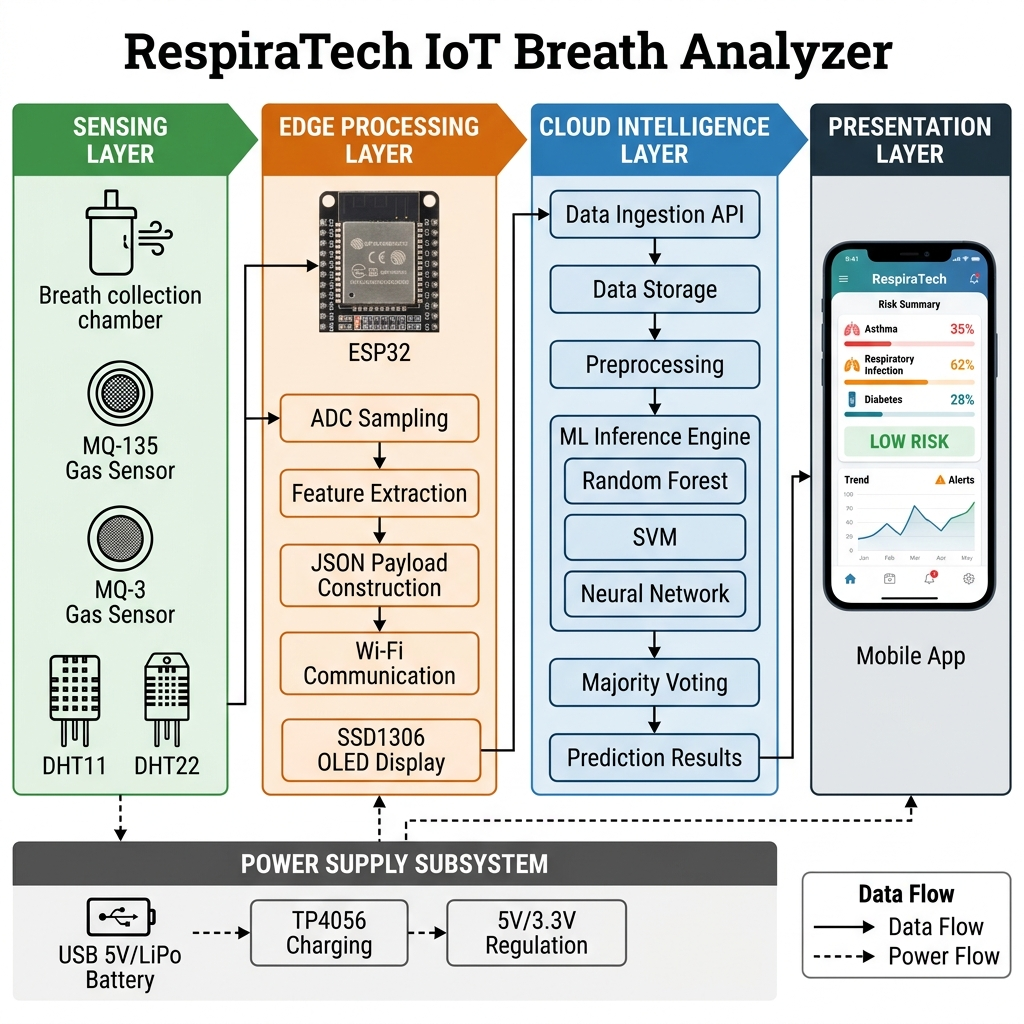
\includegraphics[width=\textwidth]{images/system_architecture.png}
\caption{System Architecture Diagram -- RespiraTech Intelligent IoT and AI-Based Breath Analyzer}
\label{fig:system_architecture}
\end{figure}
